	\section{Глобальная теорема Кронекера}

	\subsection{Группа и поле инерции для максимального идеала в случае числового поля}

	Пусть $K$~--- числовое поле (т.е. конечное расширение $\Q$), $L/K$~--- расширение Галуа с группой Галуа $G = \Gal(L/K)$.

	Пусть $\fp$~--- максимальный идеал в $\cO_L$, а $\fP$~--- такой максимальный идеал в $\cO_L$, что $\fP \cap \cO_K = \fp$. 

	В случае расширения Галуа мы знаем, что у всех идеалов, висящих над $\fp$ одинаковые индексы ветвления и степени инерции, то есть справедлива формула $e f r = n$, где 
	\begin{itemize}
	 	\item $e = e(\fP/\fp)$~--- индекс ветвления, 
	 	\item $f = f(\fP/\fp)$~--- степень инерции, 
	 	\item $r$~--- колиество максимальных идеалов в $\cO_L$, висящих над $\fp$.
	 \end{itemize} 

	 Введём такие обозначения 
	 \begin{itemize}
	 	\item $G_{\fP} = \{ \sigma \in G \ \vert \ \sigma \fP = \fP \}$. 
	 	\item $\Bbbk\lr*{\fP} = \cO_L/\fP$, $\Bbbk\lr*{\fp} = \cO_K/\fp$.
	 \end{itemize}

	 \begin{lemma} 
	 	$G_{\fP} \twoheadrightarrow \Gal\lr*{\Bbbk\lr*{\fP}/\Bbbk\lr*{\fp}}$.
	 \end{lemma}
	 \begin{proof}
	 	Так как можно заменить $K$ на $Z_{\fP}$  и доказывать, что $G_{\fP} \twoheadrightarrow \Gal(\Bbbk\lr*{\fP}/\Bbbk\lr*{\fP \cap \cO_{Z_{\fP}}})$, достаточно доказывать это рассуждение когда $G_{\fP} = G$.

	 	Соотвественно, покажем, что $\Bbbk\lr*{ \fP \cap \cO_{Z_{\fP}} } = \Bbbk(\fp)$, а для этого докажем, что $f\lr*{\fP \cap \cO_{Z_{\fP}} /\fp } = 1$. 

	 	Положим $e' = e(\fP \cap \cO_{Z_{\fP}}/\fp)$, $f' = f\lr*{\fP \cap \cO_{Z_{\fP}/\fp}}$. Так как $G_{\fP}$ действует на $\fP$ тривиальн, над $\fP \cap \cO_{Z_{\fP}}$ есть ровно один максимальный идеал, откуда $\fP$, откуда $e' f' = |G_{\fP}|$. Соотвественно, 
	 	\[
	 		e = e' e_1, \ f = f' f_1, \quad e_1 = e(\fP \cap \cO_{Z_{\fP}}/\fp), \ f_1 = f(\fP \cap \cO_{Z_{\fP}}/\fp). 
	 	\]
	 	Так как $r e f = n$, мы получаем $r e_1 f_1 = r \implies e_1 f_1 = 1 \implies f_1$. 

	 	Теперь мы считаем, что $G = G_{\fP}$. Заметим, что 
	 	\[
	 		\Bbbk(\fP) = \Bbbk(\fP)(\theta).
	 	\]
	 	Пусть $\overline{g}$~--- минимальный многочлен для $\overline{\theta}$, а $f$~--- минимальный многочлен для $\theta$. Тогда $\overline{f} \divby \overline{g}$. 

	 	\[
	 		f(x) = \prod_{\sigma \in G}(x - \sigma \theta)  \implies \overline{f}(x) = \prod_{\sigma \in G} (x - \overline{\sigma \theta}), \ \overline{g}(x) = \prod_{\sigma \in \Gal(\Bbbk\lr*{\fP}/\Bbbk\lr*{\fp})} (x - \sigma \overline{\theta}). 
	 	\]

	 	Теперь пусть $\overline{\theta} \in \Gal(\Bbbk(\fP)/\Bbbk(\fp))$, тогда $\overline{\theta}(\overline{\theta}) = \overline{\tau(\theta)}$, где $\tau \in G$. Тогда $\overline{\tau} = \overline{\sigma}$.

	 \end{proof}

	 Посмотрим тогда на короткую точную последовательность
	 \[
	 	1 \to I_{\fP} \to G_{\fP} \to \Gal\lr*{\Bbbk\lr*{\fP}/\Bbbk\lr*{\fp}} \to 1
	 \]
	 точна и рассмотрим подрасщирения, которые соотвествуют этим группам 
	 \begin{center}
	 	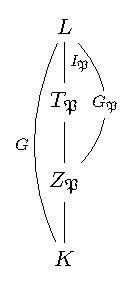
\includegraphics{lectures/6/pictures/cd_44.pdf}
	 \end{center}

	 Заметим, что $[G : G_{\fP}]$~--- количество элементов в орбите действия $G$ на $\fP$ (так как индекс стабилизатора равен размеру орбиты действия), то есть $[Z_{\fP} : K] = r$.  С другой же стороны, 
	 \[
	 	\left\lvert G_{\fP} : I_{\fP} \right\rvert = \left|\Gal\lr*{\Bbbk\lr*{\fP}/\Bbbk\lr*{\fp}}\right| = \left[ \Bbbk\lr*{\fP} : \Bbbk\lr*{\fp} \right] = f \implies [T_{\fP} : Z_{\fP}] = f.
	 \]
	 Отсюда получаем, что $|I_{\fP}| = [L : T_{\fP}] = e$. Покажем, что 
	 \[
	 	e\lr*{\fP \cap \cO_{T_{\fP}}/\fp} = 1,
	 \]
	 для этого покажем, что $e(\fP/\fP \cap \cO_{T_{\fP}}) = e$. Так как $I_{\fP} \subset G_{\fP}$, он действует на $\fP$ тривиально. Тогда нам остаётся доказать, что $f(\fP/\fP \cap \cO_{T_{\fP}}) = 1$, что равносильно тому, что группа Галуа $\Gal(\Bbbk(\fP)/\Bbbk(\fP \cap \cO_{\fP}))$ тривиальна. 

	 Запишем для расширения $L/T_{\fP}$ точную последовательность, как для расширения выше, из неё получим, что $\varphi: I_{\fP} \twoheadrightarrow \Gal(\Bbbk(\fP)/\Bbbk(\fP \cap \cO_{\fP}))$. С другой стороны, есть такая коммутативная диаграмма:\footnote{(тут я подразумеваю, что $\varphi$ это в точности композиция нужных стрелок)} 
	 \begin{center}
	 	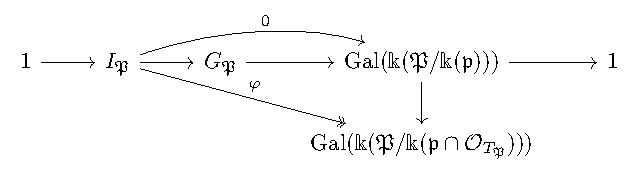
\includegraphics{lectures/6/pictures/cd_45.pdf}
	 \end{center}
	 из которой получаем, что $\Gal(\Bbbk(\fP)/\Bbbk(\fP \cap \cO_{\fP})) = e$. 


	 \begin{definition} 
	 	$I_{\fP}$ называется группой инерции идеала $\fP$, а $T_{\fP}$~--- полем инерции идеала $\fP$. 
	 \end{definition}

\subsection{Глобальная теорема Кронекера}

	 \begin{theorem}[Глобальная теорема Кронекера] 
	 	Пусть $F$~--- абелево расширение поля $\Q$. Тогда $F \subset \Q(\zeta_{n})$ для некоторого натурального $n$.
	 \end{theorem}

	 \begin{proof}
	 	Рассмотрим произвольное абелево расширение, построим для него $L \Q_p / \Q_p$ и для начала поясним, что это вообще такое. Под этим мы подразумеваем вот такой композит: 
	 	\begin{center}
	 		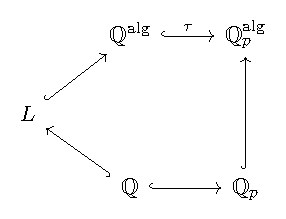
\includegraphics{lectures/6/pictures/cd_47.pdf}
	 	\end{center}

	 	Ясно, что в таком случае $L \Q_{p}/\Q_{p}$~--- расширение Галуа и 
	 	\[
	 		\Gal(\tau(L)\Q_p/\Q_p) \hookrightarrow \Gal(L/\Q), 
	 	\]
	 	откуда ясно, что это расширение абелево. Совершенно ясно, что эту конструкцию мы используем, чтоб свести глобальную теорему Кронекера к локальной. Теперь преступим непосредственно к доказательству. 

	 	Заметим, что существует лишь конечное число простых $p$, разветвлённых в $F$. Пронумеруем их: $p_1, p_2, \ldots, p_s$. По локальной теореме Кронекера каждого $p_i$ существует $n_{p_i}$ такое, что 
	 	\[
	 		\Q_{p_i} \hookrightarrow \Q\lr*{\zeta_{n_{p_i}}}.
	 	\]
	 	Рассмотрим $n = n_{p_1} \cdot \ldots \cdot n_{p_s} = q_1^{a_1} \cdot \ldots \cdot q_t^{a_t}$ и расширение $K = \Q(\zeta_n)$. Ясно, что расширение $K/\Q$~--- абелево. Докажем, что 
	 	\[
	 		F \hookrightarrow K.
	 	\]
	 	Точнее, мы покажем, что $L = KF = K$, откуда это будет следовать. Начнём с того, что покажем, что 

	 	\[
	 		e_{p_i}\lr*{L/\Q} = e_{p_i}(L \Q_{p_i}/\Q_{p_i}).
	 	\]
	 	
	 	Так как $\Q_{p_i}$~--- локальное поле, у нас существует единственное продолжение нормирования на $L \Q_{p_i}$, обозначим его за $\v_i$. Заметим, что так как $L/\Q$~--- расширение Галуа, индекс ветвления равен значению \bf{любого} продолжения нормирования, соответствующего максимальному идеалу. Например, 
	 	\[
	 	 	e_{p_i}(L/\Q) = \v_i\vert_{L}(p_i).
	 	 \] 
	 	 С другой стороны, мы знаем, что 
	 	 \[
	 	 	e_{p_i}(L \Q_{p_i}/\Q_{p_i}) = \v_i(p_i), \quad \v_i\vert_{L}(p_i) = \v_i(p_i).
	 	 \]
	 	 Таким образом, 
	 	 \[
	 	 	e_{p_i}(L \Q_{p_i}/\Q_{p_i}) = e_{p_i}(L/\Q). 
	 	 \]

	 	 Справедливости ради, тут надо пояснять, почему сужение нормирования будет нормированием. Это следует из того, что $L$ плотно в $L \Q_p$. 


	 	 Теперь заметим, что так как $F \Q_{p_i} \subset K \Q_{p_i}$:
	 	 \[
	 	 	L \Q_{p_i} = K F \Q_{p_i} = K \Q_{p_i} \cdot F \Q_{p_i} = K \Q_{p_i}.
	 	 \]
	 	 Соответственно, отсюда 
	 	 \[
	 	 	e_{p_i}\lr*{K \Q_{p_i}/\Q_{p_i}} = e_{p_i} \lr*{L \Q_{p_i}/\Q_{p_i}} = e_{p_i}(L/\Q) > 1.
	 	 \]
	 	 С другой стороны, 
	 	 \[
	 	 	e_{p_i}(K/\Q) = e_{p_i}\lr*{K \Q_{p_i}/\Q_{p_i}} = \varphi(q^{a_j}) \text{ если } p_i = q_j.
	 	 \]

	 	 Значит, $p_i$ разветвлено в $K = \Q(\zeta_n)$, откуда $n \divby p_i$, откуда 
	 	 \[
	 	 	\{ p_1, \ldots, p_s \} \subset \{ q_1, \ldots, q_t \}
	 	 \]
	 	 С другой стороны, если для некоторого $j$ мы имеем $q_j \notin \{ p_1, \ldots, p_s \}$, то 
	 	 \[
	 	 	e_{q_j}(L/\Q) = e_{q_j}\lr*{L \Q_{q_j}/\Q_{q_j}} = e_{q_j} \lr*{F\Q_{q_j} \cdot K \Q_{q_j}/ \Q_{q_j}} = e_{q_j}(K \Q_{q_j}/\Q_{q_j}) = \varphi(q_{j}^{a_j}),
	 	 \]
	 	 так как 
	 	 \begin{center}
	 	 	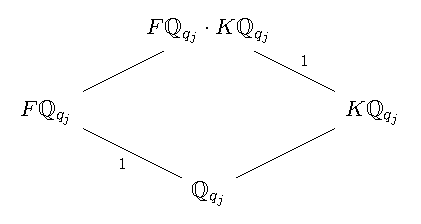
\includegraphics{lectures/6/pictures/cd_48.pdf}
	 	 \end{center}

	 	 где на стрелочках подписаны индексы ветвления. Аналогично, если $p \notin \{ q_1, \ldots q_t \}$, то 
	 	 \[
	 	 	e_p(L/\Q) = e_p(K/\Q) = 1.
	 	 \]

	 	 Рассмотрим для каждого $j$ $L_j/\Q$~--- поле инерции для $q_j$, соответственно $L_j \subset L$, притом 
	 	 \[
	 	 	[L : L_j] = e_{q_j}(L/\Q), \quad e_{q_j}(L_j/\Q) = 1.
	 	 \]
	 	 Тогда рассмотрим $S = L_1 \cap \ldots \cap L_t$. Заметим, что все простые числа неразветвлены в $S$, так как если $p \in \{ q_1, \ldots, q_t \}$, то 
	 	 \[
	 	 	e_{q_j}(L_j/\Q) = 1,
	 	 \]
	 	 а если $p \notin \{ q_1, \ldots, q_t \}$, то $e_p(L/\Q) = 1$ (так как тогда $p$ не разветвлено в $L$, а $L_j \subseteq L$). Тогда, как мы видели в первой части курса, $L_1 \cap \ldots \cap L_t = \Q$. 

	 	 С другой стороны, 
	 	 \[
	 	 	[L : L_1 \cap L_2] \le [L : L_1] \cdot [L : L_2] \implies [L : L_1 \cap \ldots \cap L_s] \le \prod_{i = 1}^{t}[L : L_i] = e_{q_j}(L/\Q) = \varphi(q_j^{a_{j}})
	 	 \]
	 	 и тогда по мультипликативности функции Эйлера $[L : \Q] \le \varphi(n)$, но так как $L \supset K$, а $[K : \Q] = \varphi(n)$, мы получили, что $L = K$. 
	 \end{proof}




	 






	 

